\documentclass[man,floatsintext]{apa6}

\usepackage{xfrac}
\usepackage{textcomp}
\usepackage[american]{babel}
\usepackage[utf8]{inputenc}

%\usepackage[compact]{titlesec}
\usepackage{tabu}
\usepackage{amssymb,amsmath}
\usepackage{setspace}

\usepackage[hyphens]{url}
%\usepackage{hyperref}
%\usepackage{breakurl}

\usepackage{subfigure}
\usepackage{graphicx}
\usepackage[group-separator={,}]{siunitx}
\RequirePackage[l2tabu, orthodox]{nag}
\graphicspath{{./figures/dissertation/}} % Specifies the directory where pictures are stored

\usepackage{csquotes}
\usepackage[style=apa,sortcites=true,sorting=nyt,backend=biber,doi=false,uniquename=false]{biblatex}
\DeclareLanguageMapping{american}{american-apa}
\addbibresource{bibliography.bib}

% Needed to ensure periods are placed at the end of every bibliography entry in the references section
\AtEveryBibitem{\clearfield{doi}}

% Make sure only urls that are printed in references section are for webpages
\AtEveryBibitem{
  \ifentrytype{misc}{}{
    \clearfield{url}
  }
}

% ref: http://tex.stackexchange.com/questions/128592/remove-backslashes-from-url-fields-in-bib-entry
\DeclareSourcemap{
  \maps[datatype=bibtex]{
    \map{
      \step[fieldsource=url,
	match=\regexp{\\},
      replace=\regexp{}]
    }
  }
}


% If the toc is too detailed, try limiting the depth of printed sections in the TOC:
%\setcounter{tocdepth}{2}

\title{FIXME}
\shorttitle{}

\author{Clayton Stanley}
\affiliation{Rice University}

\leftheader{Beitzel}

\abstract{
  FIXME
}

\keywords{FIXME}

\begin{document}
\maketitle

\tableofcontents
\newpage

\section{Motivation}

Social media sites such as Twitter, Facebook, StackOverflow, Google+, and Yelp, are composed almost entirely of human-generated content.
The amount of human-generated content on these sites is staggering, and continues to grow.
Users of Twitter's microblogging service, for example, generate half a billion tweets per day \parencite{TwitterReport2012}.
However, a single user of a social media site is most likely interested in only a small fragment of this large amount of information.
One general question to support the user in this domain is:
How can we quickly and effectively connect users to the content that they care about?

% FIXME: Fix cite for Bauer2012
One traditional technique is to provide the user with a powerful search engine so that they can actively look for content that interests them.
However, users are not forming the same search queries that work so effectively on search engines like Google.
A growing number of users on social media sites are searching for information that is happening now, in real time \parencites{Bauer2012,Jansen2011}.
In other words, users on social-media sites want the fresh \emph{stream} of information about a particular topic.
This can certainly be seen in the main user-interface views that these social media site provide:
Twitter's homepage showing your followers' tweets, Facebook's homepage showing your friends' posts, StackOverflow's daily digest of posts for particular tags, etc.

So how can we ensure that users are connected to the information streams that they care most about?
One promising approach is to model and predict the user's goals when using and searching these social media sites \parencite{Rose2004}.
If we have a better understanding of a user's goals, then we can tailor the information streams provided to the ones that are most in line with these goals.
For example, Twitter might suggest other users and hashtags for the user to follow, Facebook could suggest pages to like, Yelp could recommend businesses to check out, etc.
Researchers are currently looking for ways to automate the goal-identification task for more general search queries like those generated for Google \parencites{Jansen2008}{Lee2005}.

However, social media sites have an advantage for identifying user goals over traditional search engines:
human-generated content.
Twitter does not have only the tweet that a user is currently composing to try and identify that user's goals.
Rather, the site has all of the user's previously-generated content, and can use that information to provide a much better prediction of a user's goals.
Further, sites like Twitter, StackOverflow, Google+, and Facebook support ways for the user to explicitly identify their precise goals when creating content: Hashtags.
These user-created hashtags are a key indicator to a user's goals on a social media site. 

These hashtags relate to a user's goals and interests because they are human-generated content, and a form of human-based document tagging \parencite{Chang2010}.
Further, people are using hashtags as a way to create information streams on social media sites \parencite{Kwak2010}.
Twitter users, for example, commonly create hashtags for upcoming political events, such as debates and races \parencite{Diakopoulos2010}.
So if we can predict what hashtags a user is interested in, we have a better understanding of the information streams that they care about.
With that understanding, we can tailor the system to suggest hashtags that they may not yet know about but are of likely interest to them.
We can help aid in their discovery of fresh and relevant information that match their goals on the site.

\subsection{Research Questions}

The core research question we are interested in is:
What kinds of cognitively-plausible models can best predict the human-generated tags that a user on a social media site is interested in?
This question can be tested by generating a prediction for the most likely used hashtag whenever a user is about to generate a hashtag, and then comparing the user's chosen hashtag to the model's prediction.
This process can be framed as a memory retrieval problem.
That is, each user on a social media site has created content that contain a set of human-generated tags within the context of each post.
The process of suggesting a relevant hashtag to a user can be thought of as a memory retrieval request for a hashtag, given prior hashtag use and current context.

Co-occurrence-based modeling has been shown as a potentially useful approach when predicting Twitter hashtag use \parencite{Efron2010}.
Several memory retrieval models are based on this broad methodology, where a count is maintained of the times each contextual element (such as a word in a post) co-occur with a tag.
Two of the current state-of-the-art memory models are based on a co-occurrence methodology, and we'll be comparing these two models for hashtag prediction:
ACT-R's declarative memory retrieval theory and random permutation vector-based memory systems.

\subsubsection{StackOverflow and Twitter Task Domains}

We will compare these two memory systems across two domains where users generate tags for posts: Twitter and StackOverflow.
Twitter is a microblogging service where users create 140 character tweets and broadcast those messages out to the users who follow their posts.
A user is free to annotate important concepts or words in the tweet by preceding words with hashtags ``\#''.
User-created hashtags on Twitter are embedded into the tweet, and can be used to connect the tweet to other tweets about the same topic through common hashtag use.
After the tweet is created the hashtags become hyperlinks, and if clicked on will take a user to a summary feed of all of the tweets across Twitter that have used that hashtag.
Some recent and often-used hashtags for Twitter are \emph{\#photography}, \emph{\#startup}, \emph{\#4change}, \emph{\#android}, and \emph{\#solar}.

\begin{figure}[!htbp]
  {%
    \setlength{\fboxsep}{0pt}%
    \setlength{\fboxrule}{1pt}%
    \hfill
    \subfigure[]{\fbox{
\includegraphics[width=8cm]{twitterTweetExample1-crop.pdf}}}
    \hfill
    \subfigure[]{\fbox{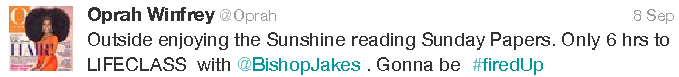
\includegraphics[width=8cm]{twitterTweetExample3-crop.pdf}}}
    \hfill
    \vfill
    \hfill
    \subfigure[]{\fbox{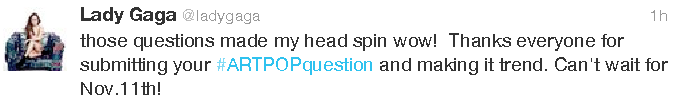
\includegraphics[width=8cm]{twitterTweetExample4-crop.pdf}}}
    \hfill
    \subfigure[]{\fbox{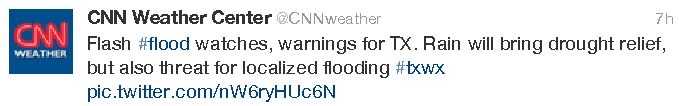
\includegraphics[width=8cm]{twitterTweetExample5-crop.pdf}}}
    \hfill
    \caption{Example tweets on Twitter.com}
    \label{figTweetExample}
  }%
\end{figure}

Some example tweets on Twitter are included in Figure \ref{figTweetExample}.
Note how users both add hashtags to the end of a tweet as a summary of the message and emphasize important concepts words in the tweet by turning them into hashtags.
That is, hashtags are both intermixed within the words of the tweet and added to the end of the message.

StackOverflow is a question and answer site for computer programming where users ask programming-related questions and fellow members of the community provide answers.
A user with a programming-related question creates a post with their question and tags the post with a few specific programming-related tags. 
User-chosen tags on the StackOverflow site represent the primary topic of the question, such as a specific programming language, tool, software package, or framework.
Some example tags for StackOverflow are \emph{PHP}, \emph{Arrays}, \emph{MVC}, \emph{C\#}, or \emph{Common Lisp}.
 
% FIXME: Use vector-graphics for this figure 
\begin{figure}[!htbp]
  \scalebox{.8}{\resizebox{\linewidth}{!}{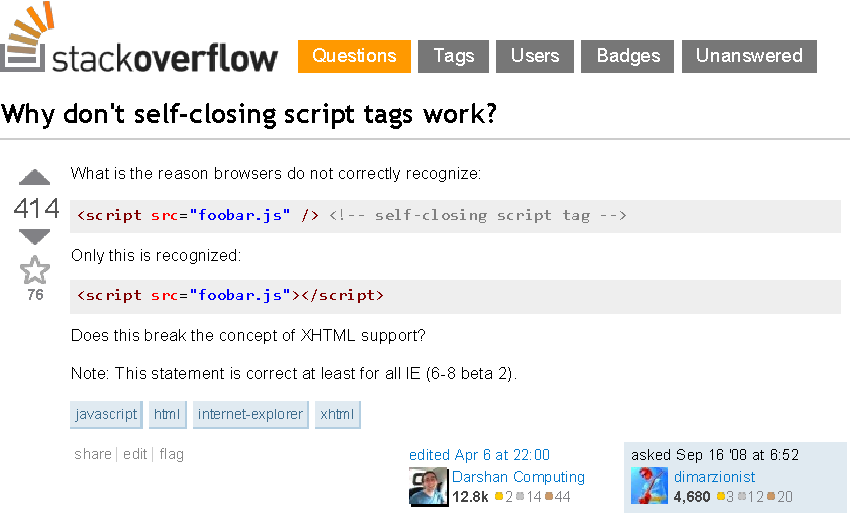
\includegraphics{stackoverflowPostExample1-crop.pdf}}}
  \caption{Example post on stackoverflow.com}
  \label{figSOExample}
\end{figure}

An example StackOverflow post is included in Figure \ref{figSOExample}.
The site requires that for each post, the user must associate at least one tag with the post.
The author used 4 tags for this post: \emph{javascript}, \emph{html}, \emph{internet-explorer}, and \emph{xhtml}, and the average number of tags per post is around 3.

These two datasets were chosen because the content of the human-generated content is quite different between them, and we are interested in retrieval models that generalize across different task domains.
However, they are also quite similar on several accounts:
Both domains have amassed large amounts of user-generated content, users generate tags for posts when creating content on the site, and the user data from the datasets are publicly available for analysis.

Also, studying user-based tag generation on these sites is a relevant task domain.
Models that can accurately predict the tags that users will generate on Twitter and StackOverflow can be used as the foundation for recommendations systems on these very popular sites.
These systems can help newer users by recommending proper tags for their newest content.
On the StackOverflow site for example, experts often subscribe to specific hashtags that interest them, and receive a daily digest of posts that are tagged with those hashtags.
Helping the user properly tag posts on StackOverflow ensures that right community sees the post, which greatly increases the chance that the question on the post will be answered quickly and correctly.
For Twitter, hashtags represent streams of information that are possibly interesting to the user.
Having a recommendation system that can suggest relevant hashtags to the user provides a way for the user to connect to and discover new information streams.

\subsubsection{Comparison Between ACT-R and Vector-Based Memory Systems}

ACT-R's declarative memory and vector-based memory systems are substantially different in their implementation.
Nonetheless, both can successfully model the classic fan effect phenomena found in word pairing experiments \parencite{Rutledge2008}.
We will extend the work done by \textcite{Rutledge2008} by formally comparing the models on large-scale hashtag prediction tasks.
We'll also replace the vector-based model used by \textcite{Rutledge2008} with an improved and simplified random-permutation model \parencite{Sahlgren2008}.
The primary objective is to compare the random-permutation vector-based model to ACT-R's declarative memory theory.

An advantage of vector-based models is that word order can be easily incorporated into the single co-occurrence representation \parencite{Jones2007}.
Word-order information on sites like Twitter may contain highly-predictive pieces of information, as it is likely that specific words immediately precede specific hashtags.
However, it is unclear and unexplored how word order can be represented in the ACT-R declarative memory theory.
We will explore how the word-order strength of vector-based models can be incorporated into the ACT-R theory when testing the models on hashtag prediction tasks.

ACT-R's declarative memory system has a strong theory on how a user's prior knowledge and experience influences the likelihood that a particular memory item is retrieved \parencite{Anderson2004}.
However, it is unexplored how a user's prior knowledge should influence retrieval for vector-based models.
We will explore how a user's prior knowledge influences the likelihood that a particular hashtag is generated for both ACT-R's memory theory and vector-based models.

\subsubsection{Lifetime of a Hashtag for a Specific User}

Prior research has examined the growth and decay cycle of hashtag use across users \parencite{Tsur2012}.
However, much less is known about hashtag lifetime within a single user.
It may not be the case that a hashtag's life cycle for a single user matches the life cycle across users.
Further, modeling a hashtag's life within users is much more applicable to hashtag prediction, since that model can be directly incorporated into a specific user's prior likelihood of hashtag use.
So we will characterize the hashtag growth and decay cycle within users.
The expectation is that this cycle will match ACT-R's decay rate used in the declarative memory system to compute a particular memory item's prior.
This decay rate equation formalizes how recency and frequency of hashtag use relate to the prior probability that a hashtag will be retrieved.

\subsubsection{User-Customized Hashtag Prediction}

The end goal of this work is to identify a memory retrieval model that can suggest relevant hashtags to users when they wish to retrieve one.
These hashtags should be customized to their specific interests and relevant to the content of the post that they are currently creating.
This will undoubtedly require a combination of two primary model components:
[1] A user's prior likelihood of choosing a particular hashtag, given their previously-generated content, and [2] the likelihood that a particular hashtag is related to the context of the post being generated. 

A user's prior hashtag use will be an essential model component for domains such as Twitter, where the number of possible hashtags is practically infinite.
In these domains, the model can utilize a user's prior hashtag use as a way to prune the infinite space of possible hashtags, and generate a much smaller and more manageable set for prediction.
However, not only should the model properly take into account a user's prior hashtag use, but it should also generate new hashtag predictions when a user is most likely choosing a hashtag they have never used before.
Calibrating the models to properly balance this exploitation of prior hashtag use versus exploration of new hashtags will be a primary research focus.
The end goal is to have a model that can properly balance the user's prior tag with the contextual cues in the post in order to generate an accurate prediction.

\section{Prior Research}

\subsection{Recommendation Systems}

A model that predicts a user-chosen hashtag is a specific type of the more general recommendation systems.
These systems have grown in need with the growth of the web.
Users on a site need quick access to specific pieces of information, and the site contains much more information than they can process or care about.
Recommendation systems are used to tailor the information presented to what is most relevant to the user \parencite{Pazzani2007}.

\subsubsection{The Netflix Prize}

% FIXME: Fix cite for Bennett2007
The Netflix Prize \parencite{Bennett2007} is an example of a recommendation system where prior user behavior and current context was used to present the most relevant information to the user.
Netflix is an online-subscription service where users can stream their favorite television episodes and movies.
Each user of the site is only interested in a small portion of the entire library of content that Netflix provides.
In order to provide a high-quality user experience on the site, Netflix created a content-recommendation service.
This tool recommends to the user movies and television episodes that most likely match their specific interests.
Netflix wanted to improve the accuracy of their recommendation system, so they held a competition where teams could try to improve on the accuracy of the service.

The winning team utilized a singular value decomposition (SVD) method to identify particular dimensions of the entire content library (e.g., genre, time period, previously watched) that best predicted user preferences.
This is a dimensionality-reducing technique that aims to filter out noise by forcing the data to be represented from a smaller number of dimensions than were originally present.
This method used prior user behavior to classify a user along the dimensions of the reduced space, and current user behavior (e.g., just watched) to understand what they were interested in watching at that moment.
By using an SVD technique and combining these indicators, the model improved on Netflix's original recommendation system by 10\%.

\subsubsection{Recommending Followers on Twitter}

Recommendation systems based on the content of user-generated posts have been successful in recommending people on Twitter for a user to follow.
\textcite{Hannon2010} built a Twitter follower recommendation system by creating a profile of each user based on the words they used in previous posts.
The recommendation system would then suggest other Twitter users to follow that had similar profiles to a particular user.
The profiles were created by generating a word frequency matrix of words x (user + followers + followees), and then providing that matrix as input into the Lucine text search engine framework.
When the system needed to recommend a set of individuals for a user to follow, it would take all of the words used in posts from that user to construct a search query to be provided to Lucine.
That search query would return the most likely users that share similar words in posts within their twitter network with the words provided in the query.
Using this simple technique based on a standard text search engine allowed the recommendation system to accurately predict the people that a particular user will follow at 25\% accuracy.

\subsubsection{Hashtags for Recommendation Systems}

\textcite{Efron2010} showed how hashtags might be used as a type of recommendation system for Twitter.
Users constructed a query of text that represented a search for a topic that they were interested in.
The system then retrieved the most likely hashtags that were associated with that search query.
The model is based on building a word co-occurrence matrix of words x hashtags, and then uses that matrix to assign a similarity score for each hashtag when provided with a search query.
Participants graded how relevant the hashtags returned were to each search query.
The results suggest that hashtags contain useful information that help classify the gist of a post. 
Although this model does not predict hashtags directly when composing a tweet, a model like this could certainly be tailored for that purpose.

\subsection{Hashtag Prediction}

More specific hashtag-recommendation models that attempt to predict a user's chosen hashtag have also been created and tested for a few social media sites.
Google has even deployed a hashtag-recommendation model to help users properly tag posts for their Google+ social media site \parencite{GoogleKeynote2013}.
However, to our knowledge a hashtag-recommendation model for Twitter tweets has not yet been attempted.

\subsubsection{StackOverflow}

\textcite{Kuo2011} was the first to model tag use for StackOverflow posts.
His set of models were originally designed for next-word prediction for large text document collections.
In order to structure the models to work for StackOverflow tag prediction, the models would request the most-likely next word after a user generated a post, and restrict the space of possible words to only tags.
He tested the set of next-word prediction models to generate predictions for the most likely tags that a user would choose when asking a question on the site.
Interestingly, the Bayesian co-occurrence model outperformed the more complicated and computationally expensive Singular Value Decomposition and K-nearest-neighbors models.
This model can accurately predict a user-chosen tag at 47\% accuracy.

\textcite{Stanley2013} also modeled a user's chosen tags for a post on the StackOverflow site.
The model was based on ACT-R's declarative memory retrieval theory, which at the core is also a Bayesian co-occurrence model.
However, this model scaled much better than the co-occurrence model presented in \textcite{Kuo2011}.
Because of this, 100 times more posts were used to build the co-occurrence matrix (\num{1000000} versus \num{10000}), which significantly increased the model's performance.
After scaling up the model, this model can successfully predict a user's tag for a post at 65\% accuracy.
It is interesting that in both research papers the best performing model was based on a Bayesian co-occurrence framework, since that is precisely the framework from which ACT-R's declarative memory system is built.
This suggests that more cognitively-plausible memory retrieval models may outperform more general machine-learning approaches in this particular task domain:
predicting the user-chosen tags for human-generated content on social media sites.

A tag suggestion tool has also been deployed for the \url{http://tex.stackexchange.org} site. \parencite{LatexTags2013}
Both the \LaTeX site and StackOverflow are part of the broader StackExchange network of question and answer sites, and they provide the same user interface and workflow when asking questions.
Once a user has created a question on the Latex site, the site provides subdued text of suggested tags in the text field where the user fills in the tags to associate with the question.
The post author is not forced to use the suggested tags, and is free to choose tags from them or tags not represented in the suggested set.

The Latex site is not nearly as popular as StackOverflow currently.
The site has roughly \num{50000} questions compared to \num{5000000} questions on StackOverflow.
It may be the case that the StackExchange company decided to try out a tag recommendation system on one of their smaller sites first, before deploying this type of system on their most popular StackOverflow site.
Or it is possible that their current tag recommendation system is not efficient enough to work with the demand of the StackOverflow site.
Nonetheless, it is encouraging that StackExchange finds tag recommendation models beneficial enough to the user to start adding them to their question and answer sites. 

\subsubsection{Google+}

The hashtag recommendation system deployed for the Google+ microblogging service is probably the most ambitious model of user-created hashtags to date \parencite{GoogleKeynote2013}.
The user interface for this recommendation system for an example Google+ post is shown in Figure \ref{figGoogle+Hashtags}.

\begin{figure}[!htbp]
  \scalebox{.4}{\resizebox{\linewidth}{!}{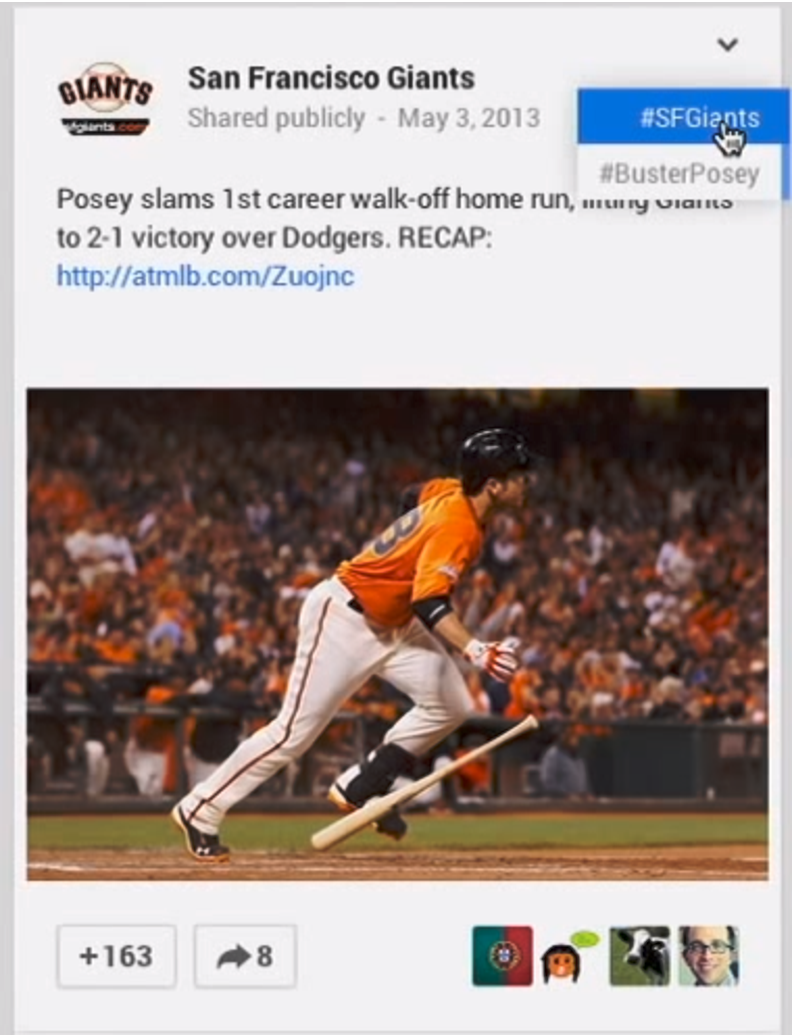
\includegraphics{google+HashtagExample-crop.pdf}}}
  \caption{Example post on Google+. The system recommended \emph{\#SFGiants} and \emph{\#BusterPosey} as hashtags for the user-generated post}
  \label{figGoogle+Hashtags}
\end{figure}

The workflow and user interface provided for recommending hashtags for Google+ is similar to how a hashtag recommendation system for Twitter might look.
When generating content on Google+, the system automatically associates the most likely relevant hashtags with that post.
The user is free to remove any or all of the tags that the system has associated with the post, and can also use tags that were not included in the recommended set.

Google is apparently highly confident in the accuracy of their system.
On the Latex site, the User Interface provides subdued suggestions to the user, but requires the user to explicitly choose each tag he/she wants to associated with the post.
For Google+, the User Interface automatically provides tags for a user's post, and then requires the user to explicitly change those tags if he/she wants to use a different set.
If tag accuracy is high enough, the Google+ technique is certainly favorable, since the user does not have to spend time figuring out which tags best represent this post.
However, if the model makes even just a few errors, users may become annoyed and frustrated with the recommendation system, since they will have to explicitly correct it every time they generate a post.

\subsubsection{Twitter}

Several hashtag recommendation models for Twitter have been developed recently.
One of the first models used a Bayesian co-occurrence statistical technique to predict the most likely hashtag associated with a post as a function of prior hashtag use and context. \parencite{Mazzia2009}
The model present by \textcite{Mazzia2009} is very similar to an ACT-R declarative retrieval model.
The main potential difference is that the global prior likelihood of a hashtag is computed without taking into account the specific user's past history.
Instead, the global prior is an overall average frequency of hashtag use.

Several other models have taken a tweet-centered approach to hashtag prediction, where suggested hashtags are collected from hashtags used from similar tweets.
\textcites{Li2011, Zangerle2011, Kywe2012} all store a content vector for each tweet, and then compute a word co-occurrence-based similarity score between a composed tweet and the rest of the tweets in the database.
\textcites{Zangerle2011, Kywe2012} use the Apache Lucine infrastructure to compute the similarity score, while \textcite{Li2011} uses a custom similarity score derived from the WordNet database to compute similarities.
Regardless of the method to compute the similarity between tweets, each method collects the hashtags used from a set of the most similar tweets, then ranks the set, and presents the top 5-10 hashtags to the user.

This tweet-centered approach is quite different than the hashtag-centered approach presented in \textcite{Mazzia2009}.
With a hashtag-centered approach, a direct association is built between the words in a tweet and hashtags that occur in tweets.
With a tweet-centered approach, that association between words and hashtags is indirect:
The relationship is built between a tweet and its content, and then similar tweets are assumed to use similar hashtags.
One problem with the tweet-centered approach is that the storage size grows with the number of tweets, as a vector representation of the content in each tweet has to be maintained to later compute tweet similarity.
The storage size for a hashtag-centered approach grows with the number of hashtags, but it seems reasonable that this will grow slower than the number of tweets and asymptote after collecting a large sample of tweets.
So from the perspective of efficient information storage and retrieval, it seems more likely that the hashtag-centered approach used in \textcite{Mazzia2009} will scale as Twitter grows in size and use.

\textcite{Kywe2012} also customized their tag prediction model to the user's past hashtag use, and was one of the first to do so when developing a hashtag-prediction model for Twitter.
The set of recommended hashtags was the union of hashtags used in similar tweets and hashtags used by similar users.
This was done by storing a content vector of hashtag use for each user (user-centered approach) alongside the content vectors of hashtag use for each tweet (tweet-centered approach).
To generate recommended hashtags, the model would return the top-ranked hashtags from the hashtags used in 0-50 similar tweets and 0-4 similar users.
Prediction accuracy improved when the model combined recommendations based on hashtags in both similar tweets and the top few similar users compared to basing recommendations on similar tweets alone. 

A topics-based approach was used by \textcite{Godin2013}, where the model predicted the most likely set of topics that were associated with a tweet, and tested if these topics matched the tweet by using human raters.
The latent topics for the collection of tweets were generated using a Latent Dirichlet Allocation (LDA) statistical methodology.
This is similar to singular value decomposition in that the most likely hidden dimensions (i.e., topics) of the data are discovered by searching for reduced representations of the data that cover most of the variance. 
Human graders rated how well the models generated topics for a tweet related to the content in the tweet.
The LDA model performed well, and generated relevant topics.

However, a topic-generating model is not performing the same task as a hashtag-prediction model.
The authors argued that these general topics could be used to categorize the post, in addition to the hashtags already used by the author in the post.
It is unclear though if a user would want to label their tweet with these general topics.
Perhaps they would rather use more specific hashtags to be more precise in how they label the tweet and how that tweet is associated with tweets within the rest of the community.
In fact, they have already chosen to be more precise in the specific labels that they use for the tweet, since they chose to label the tweet with specific hashtags instead of general topics.
Now it is certainly the case that the topics generated by a latent-based model may be similar, if not identical, to the hashtags used in the post.
However, it seems a bit indirect to build a model that predicts general topics, since embedded in the data are the exact ``topics'' (i.e., hashtags) that each user chose to use for each tweet.
Why not take those topics already present in the data and build a model that produces them?
In other words, the topics data are already in the tweet, so why not use them?

\subsubsection{State of Research on StackOverflow and Twitter}

Although recent work has been done to model human tagging on the StackOverflow site, to our knowledge no vector-based holographic memory model has been tested or used.
We are curious to see the prediction difference between a vector-based models and current co-occurrence models on the StackOverflow dataset.
Both types of models are neurologically plausible, and both have been successfully incorporated as the declarative memory component of the ACT-R cognitive architecture \parencite{Rutledge2007}. 
Given that the Bayesian cognitively-plausible models have done so well to predict tag use on StackOverflow, we are curious to see how a cognitively-plausible vector-based model performs at the task.

Also, a vector-based retrieval model has not yet been tested on Twitter.
One of the advantages of vector-based models is that word order can be easily incorporated into the single co-occurrence representation \parencite{Jones2007}.
It seems quite likely that the few words used just before a hashtag embedded in a tweet will be highly predictive of the hashtag chosen.
To our knowledge, only bag-of-words models have been tested on Twitter to predict hashtags, where co-occurrence between words and hashtags are computed independently from where the word is located in the tweet.
It will be interesting to see how much (if at all) accuracy improves when incorporating word-order information into the model.

There has been a mix of co-occurrence and latent-based models created to predict hashtags use on Twitter, and the results are encouraging.
However, there has been very little research on how a specific user's past hashtag use should influence the model's prediction when that user is composing a tweet.
\textcite{Kywe2012} did take a user-centered view with their model, but the hashtags predicted by the user and content were analyzed separately and then the top from each group were combined for prediction.
The ACT-R declarative memory retrieval theory shows how past user behavior and current context combine to produce the most likely retrieval.
Each component is summed together to generate a total activation, and then the likelihood of chunks are ranked by that summed activation.
This technique allows for a more natural combination of the two components, where weights can be assigned to each component depending on how strongly each term predicts performance.
This type of weighted additive model that combines past user behavior and current tweet context to predict the most likely hashtags has not yet been explored for Twitter.

\subsection{ACT-R Declarative Memory Theory}

ACT-R \parencite{Anderson2004} is a cognitive architecture that formalizes how each cognitive process of the brain (e.g., memory, learning, visual and motor) interacts to produce behavior.
The declarative memory system is a component of that architecture that models the timing, learning, and forgetting processes that make up long-term declarative memory retrieval.
The equations that make up this system can be described through a rational analysis of long-term memory retrieval.
That is, given the task of retrieving a chunk of information from long-term declarative memory,
the current context (i.e., external and internal environment state), and past experience (i.e., prior memories and exposure), 
what is the optimal behavior (i.e., the optimal chunk to retrieve from memory)?
Using Bayesian reasoning, each chunk of information in declarative memory can be assigned a prior likelihood of being retrieved again, given the prior number of times it has been needed.
Those prior probabilities for each chunk are then adjusted for the current context, so that the posterior probabilities represent the likelihood that a chunk is needed, given prior odds and current environment state.

\subsubsection{ACT-R DM Model}

\begin{table}[!ht]
  \caption{ACT-R Declarative Memory Model}
  \label{tabACT-RModel}
  {\tabulinesep=1.2mm
    \begin{tabu}{ll}
      \hline
      Common Name &  Equation \\
      \hline
      Activation &	 	$A_{i} = B_{i} + \sum_{j \in c}^{} W_{j} S_{ji}$ \\
      Attentional Weight &	$W_{j} = \frac{W}{n}$ \\
      Base Level & 		$B_{i} = log \sum_{j=1}^{n} {t_{j}}^{-d}$ \\
      Constant Base Level &	$B_{i} = log \frac{p(i)}{p(\overline{i})}$ \\
      Strength of Association &	$S_{ji} = log \frac{p(i|j)}{p(i|\overline{j})} \approx log \frac{p(i|j)}{p(i)}$ \\
      Recall Probability &	$P_{i} = \left( 1 + e^{\frac{\tau - A_{i}}{s}} \right )^{-1}$ \\
      \hline
    \end{tabu}
  }
\end{table}

A formal description of the ACT-R Declarative Memory model is included in Table \ref{tabACT-RModel}.
The total activation ($A_{i}$) for a chunk in declarative memory is a function of two components: base level activation ($B_{i}$) and strength of association ($S_{ji}$).
The recall probability that a chunk will be retrieved from memory increases with total activation ($A_{i}$).

\subsubsection{Base-Level Activation}

Base-level activation reflects the log prior odds of needing an observed chunk again.
The primary way to calculate these log prior odds is to use the standard base level equation in Table \ref{tabACT-RModel}.
This equation formalizes how log prior odds are a function of both frequency and recency of prior exposure to a particular chunk.
Chunks used more frequently (either through exposure or from a retrieval) are more likely to be needed for retrieval again.
However, as time progresses and a particular chunk is no longer used, the activation for that chunk decays.
In this way the standard base level equation formalizes the time dynamics of the retrieval system, where a chunk's base-level activation evolves over time, depending on its current frequency and recency of use.

For some domains, it is reasonable to assume that the base-level activations of each chunk within a particular window of interest are stable, and do not change within that window.
Programming-language popularity over the past few years is a reasonable example of this.
Although the popularity of various programming languages has certainly changed slightly over the past few years (e.g., \emph{closure}'s growth), it is not the case that the changes have been drastic.
\emph{C\#}, \emph{Python}, and \emph{Java} are still a few of the most popular languages, \emph{Common Lisp} has not gained or lost much ground in popularity over the past few years, etc.

Further, if this is a reasonable assumption to make, it greatly simplifies the computation of the base-level activation for chunks, and can turn the computation into a tractable problem for large datasets.
In these time-constant domains, one can compute the log prior odds of needing each chunk directly as the log odds ratio of being exposed to a chunk.
For example, if the StackOverflow tag \emph{PHP} has been used four times as often as the tag \emph{Common Lisp}, then the prior odds of needing \emph{PHP} again is $\frac{.8}{.2}=4$ times that of \emph{Common Lisp}.

\subsubsection{Strength of Association}

Strength of association ($S_{ji}$) reflects the amount of log odds adjustment to the activation of a chunk, given the current context (i.e., external environment and internal state).
Context for the StackOverflow domain for example, can be represented as each word in the title and body of a post.
Context for the Twitter domain would be the words in a Tweet.
Association strength between a chunk in memory and a single contextual element can be computed directly by calculating its context-adjusted odds ratio:
The likelihood a chunk occurred with the current context ($p(i|j)$) over the likelihood that the chunk occurred in any of the other contexts ($p(i|\overline{j})$).
For large datasets, the likelihood that a chunk occurs in any particular context reaches near-zero values ($p(j) \Rightarrow 0$).
So it can be assumed that the likelihood that a chunk occurs in any context but one ($p(i|\overline{j})$) is equivalent to the likelihood that a chunk occurs in any context ($p(i)$).
This assumption has been both mentioned and used when deriving the $S_{ji}$ equation \parencite{Anderson1989}, as well as in recent research working with large-scale datasets \parencite{Stanley2013}.

Using this assumption for large datasets, the interpretation of the context-adjusted odds ratio becomes much simpler.
If this ratio for a particular tag and context chunk is greater than one, then the log is positive, which means that this context has been observed more often with this tag than in general.
If this ratio is less than one, then the log is negative, which provides a negative adjustment of total activation since this context has been observed more often in general than with this particular tag.

\subsubsection{Connection to Pointwise Mutual Information}

Pointwise Mutual Information (PMI) is a another co-occurrence index that measures strength of association between two terms \parencite{Farahat2004}.
It is based on the co-occurrence count between pair-wise observations of terms, similar to ACT-R's strength of association.
The PMI index is included in Equation \eqref{eqPMI}.

\begin{equation}
  \label{eqPMI}
  \mathit{PMI}(y,x) = log \frac{p(y|x)}{p(y)}
\end{equation}

Further, this PMI equation is identical to ACT-R's strength of association ($S_{ji}$) equation for large datasets.
Once the number of occurrences is large enough such that the probability of observing any particular contextual element ($p(x)$) is near zero, then ACT-R's strength of association index simplifies to the PMI equation.

\subsubsection{Scaling the Equations}

The majority of tag-recommendation systems use some measure of word pair associations to compute the likelihood of a tag, given current context.
It is important that this measure scales well enough to handle the sheer volume of information present in online social media datasets.
Large-scale social media datasets such as StackOverflow and Twitter contain on the order of millions to hundreds of millions of unique word pair associations between terms and tags.
If one wants to capitalize on all of the information present in the database to build the most accurate measure of relatedness between words and tags, then the association measure used must scale to this large size.

ACT-R's strength of association ($S_{ji}$) and the equivalent pointwise mutual information index ($\mathit{PMI}_{ji}$) have been shown to scale well for large corpora.
\textcite{Douglass2010} implemented the large-scale version of $S_{ji}$ in Erlang.
The wall-clock time required for a declarative memory retrieval request scaled linearly with the size of declarative memory with this implementation.
Retrieval times were around one second with the largest declarative memory that contained over one million associations (co-occurrence pairs).

The SNIF-ACT framework is also based on the large-scale version of $S_{ji}$, and scales well when working with a large-scale search query database for internet search \parencites{Fu2007,Pirolli2003}.
The $S_{ji}$ values were based on a 118GB local database of 10 million pages of the Stanford WebBase Project \parencite{Farahat2004}.
So this implementation did not fit into RAM, but a spinning-disk database implementation still scaled well enough for reasonably fast retrieval times for $S_{ji}$ values.

The SNIF-ACT model uses strength of association to measure the relationship between the words in a search query and the words contained in each query result.
A higher $S_{ji}$ between a query and a result means that the result is a better fit for the query, and that the user is more likely to click on that link.
The links that user chose in experimental testing were largely predictive of the strength of association measure.
The predictive power of the SNIF-ACT model went above and beyond what would be predicted by simply assuming that the user always clicks on the first link in the search results page.

\subsubsection{\textcite{Stanley2013}'s ACT-R DM Model for StackOverflow}

\begin{table}[!ht]
  \caption{The StackOverflow tag prediction model}
  \label{tabModACTRModel}
  {\tabulinesep=1.2mm
    \begin{tabu}{ll}
      \hline
      Common Name &  Equation \\
      \hline
      Activation & 		$A_{i} = B_{i} + \sum_{j\in T}^{ } W_{j} S_{ji} + \sum_{j\in B}^{ } W_{j} S_{ji} - O$ \\
      Base Level & 		$B_{i} = log \frac{p_{i}}{1-p_{i}}$ \\
      Strength Assoc. &		$S_{ji} = log \frac{p(i|j)}{p(i))} = log \frac{NN_{ji}}{N_{Row}(j)N_{Col}(i)}$ \\
      Co-occurrence &		$N_{ji} = \sum_{}^{}{observed_{ji}}$ \\
      Observations &		$N = \sum_{}^{}{\sum_{}^{}{N_{ji}}}$ \\
      Attentional Weight& 	$W_{j} = W \frac{E_{j}} {\sum_{}^{} {E_{j}}} $ \\
      Scaled Entropy & 		$E_{j} = 1-\frac{H_{j}}{H_{max}}$ \\
      Entropy & 		$H_{j} = -\sum_{i=1}^{N}p(i|j)log\left (  p(i|j) \right )$ \\
      Offset & 			$O = \frac{1}{5}\sum_{i\in top 5}^{ } A_{i}$ \\
      \hline
    \end{tabu}
  }
\end{table}

A formal description of the modified ACT-R Bayesian model from \textcite{Stanley2013} is included in Table \ref{tabModACTRModel}.
The activation of each tag ($A_{i}$) is a function of four components:
That tag's base level activation ($B_{i}$), contextual activation for the words in the title, activation for words in the body, and an offset term ($O$).
This model has been modified from the standard ACT-R model (Table \ref{tabACT-RModel}) in three ways:
Two separate contextual components were used (words in title and body of post), an offset term was added, and an entropy metric was used to compute the attentional weight ($W_{j}$).

The offset term was added to normalize the mean activation across retrievals.
This allowed the use of a logistical regression statistical technique to calibrate the weights for each of the terms.
The title and body contextual components were separated since it seemed plausible that the words in the title would be better predictors of the tag used than the words in the body.
It actually turned out that the words in the body were a better predictor of tag use \parencite{Stanley2013}, most likely because there are many more words in the body than the title of the post.
The entropy metric was used to compute the attentional weight for two reasons:
Stop words could be included in the analysis, and more predictive words of some tag (e.g., the word ``PHP'' in a post) were given higher weight.
Using an entropy metric (as opposed to weighting each word equally in the post) allows the model to allocate limited attentional resources ($W$) to important contextual elements.

\subsection{Latent Semantic Analysis Memory Theory}

Latent Semantic Analysis \parencite{Landauer1997} (LSA) is a technique that has mathematical roots in factor analysis and also measures strength of association between two terms.
The process starts with a set of N documents.
A word x document co-occurrence matrix is built by counting the number of times each word appears in each document.
The dimensionality of the full word frequency co-occurrence matrix is then reduced and forced to be represented on a smaller set of dimensions.
This process is similar to how factor analysis takes a data table and finds the most efficient way to represent that data with as few dimensions as possible.
The strength of association between two words is measured by the cosine of the two word vectors across the reduced dimension space, which would be similar to computing the cosine of two correlated eigenvectors.

Usually information is lost when the data are restructured into a smaller set of latent dimensions.
However it was shown that this process actually improves productiveness and reduces noise by allowing the frequency count of highly similar concepts (words) to be pooled together and represented by a single dimension.
They tested the LSA model on the Test of English as a Foreign Language (TOEFL) task of choosing the best of four possible synonyms to a target word.
Model results were on par with a large sample of applicants to american universities from non-English speaking countries (64.4\% compared to 64.5\%).
Model performance also improved when the original dimensionality of the data was reduced.

\subsubsection{Singular Value Decomposition}

LSA uses the Singular Value Decomposition process to reduce the dimensionality of the word x document co-occurrence matrix.
The technique attempts to maximize the amount of variability in the data left after forcing the original dimensionality of the data to be reduced.
The best way to remove a dimension while maintaining all variability is to look for words with highly-similar co-occurrence patterns and deduce that these words represent the same concept.
For example, synonyms such as \emph{\#photograph} and \emph{\#photo} would appear interchangeably across documents, so these terms would be collapsed to a single dimension and frequency counts would be pooled.
By pooling co-occurrence counts the model is able to generate better predictions with less data.

\subsubsection{Word Order}

Although the LSA model has been shown to perform well as a way to measure similarity between two terms, one of the main criticisms is that it is a ``bag of words'' model.
This means that the model does not account for or pay attention to word order when building the base word x document matrix or consequently, when performing the SVD dimension reduction.
Other models that can account for word order have been shown to perform better than ``bag of words'' models on tasks that do not even appear to require grammatical structure such as word order to do well.
For example, \textcite{Jones2007} compared a vector-based model called BEAGLE directly to LSA, training and testing both models on the same corpus used in \textcite{Landauer1997}.
The context-only BEAGLE model (no word order) performed slightly better than the LSA model at the task (55.6\% vs. 55.3\%).
However, even in a multiple-choice domain where the task is to identify synonyms (very little grammatical structure in the task), adding word order when training the model improved task performance to 57.5\%.
It seems reasonable to expect that task performance will improve much more on tasks where word order is used (e.g., generating a Twitter hashtag in the middle of a sentence).

\subsubsection{Scaling Issues}

Another issue with LSA is the SVD matrix decomposition technique is computationally very expensive.
As the size of the original word x document matrix increases, the SVD computation becomes more and more time consuming.
If the domains where LSA is being applied contained small enough datasets where SVD computation could be computed in a reasonable amount of time, then this would not be much of a concern.
However, with large-scale human-generated datasets such as Twitter, Stackoverflow, and Wikipedia, the total size of the dataset far exceeds the maximum size that can even be computed by an LSA approach.
\textcite{Budiu2007} used the first six million pages of the Stanford WebBase corpus to compare performance between LSA and PMI on the TOEFL, and the LSA model could not be implemented with this size dataset.
Instead, they compared the measures on the smaller Touchstone Applied Science Associates (TASA) corpus created from \num{60527} samples of text from high school to early college textbooks.
This is one of the available corpora on the LSA website and is aimed to summarize the general reading up to the 1st year of college \parencite{Budiu2007}.

When \textcite{Budiu2007} compared the simpler PMI (i.e., $S_{ji}$) measure to LSA on smaller TASA-corpus-size datasets, LSA performed much better (23\% vs. 60\%).
However, once the dataset surpasses in size what is computationally feasible with LSA, the much simpler PMI measure can still be computed, and the performance for PMI becomes on par and even surpasses that of LSA.
This was one of the primary motivating reasons that LSA was developed in the first place, since reduced dimensionality model out-performed the full dimensionality model on TASA-sized datasets.
\textcite{Budiu2007} also trained the PMI measure on the much larger Stanford WebBase corpus and tested the measure on the TOEFL.
This PMI model increased accuracy from 23\% to 51\% when training the dataset on the smaller TASA compared to the larger Stanford dataset.
Further, when \textcite{Turney2001} trained the PMI measure on the even larger AltaVista index of 350 million webpages, the accuracy on the TOEFL increased to 73.75\%, which is 10\% higher than the TASA-trained LSA.
This suggests that simpler models may be preferred to more complex (yet more accurate) models in large-scale domains, since the simpler models scale and can utilize all available information to generate predictions.

\subsubsection{Cost of Incremental Updating}

Another issue with LSA is that adding additional observations to an already-computed reduced representation requires rerunning the SVD \textcite{Farahat2004}.
Since computing the SVD is the most computationally-expensive operation with LSA, it is difficult to see how LSA could be implemented in incremental domains where information is periodically being added.
For Twitter and StackOverflow, it might certainly be useful to update the strength of association representation when new information arrives, especially for Twitter, where hashtag use and news content change rapidly.

\subsection{Vector-Based Memory Systems}

``holographic'' memory systems \parencite{Plate1995} or vector-based memory systems represent a concept (i.e., chunk) as a vector.
The representation of the concept is distributed across all elements of the vector.
This is somewhat similar to taking a column (i.e., a tag) on a word co-occurrence matrix and saying that the distribution of co-occurrence counts across the rows in the column is the representation of that concept.
However, vector-based memory systems represent information in a much more compact way than a full word co-occurrence matrix.

For vector-based systems, each word is represented by an environment vector $e_{j}$ that is nearly orthogonal to all other words' environment vectors.
The number of dimensions for these vectors is much less than the number of rows in a full word co-occurrence matrix, which is how vector-based systems represent information in a much more compact space.
Paired with each environment vector ($e_{i}$) is a memory vector ($m_{i}$) that contains the summed representation of all other environment vectors that have co-occurred with that $e_{i}$ environment vector.
These memory vectors can contain environment vectors from bag-of-words co-occurrence information ($c_{i}$) and word order information ($o_{i}$), which can be combined into a single representation ($m_{i}$).
Over time, memory vectors accumulate a distributed representation of the most common environment vectors that co-occurred with them.

\subsubsection{Retrieval Process}

Retrieving the most likely chunk given context can be done in two ways: decoding and resonance \parencite{Jones2007}.
Decoding takes the memory vector for context and decodes it back into an environment vector.
The cosine between that decoded environment vector and all other environment vectors is computed and ranked, and the chunk with the environment vector with the highest cosine is retrieved.
For example, assume that a user has written the word ``zend'' in a post.
``zend'' has co-occurred with \emph{PHP}, so the unordered memory vector for ``zend'' ($c_{zend}$) contains the unordered environment vector for \emph{PHP}.
Since the environment vector for \emph{PHP} was added to the memory vector for ``zend'' without any encoding, no decoding is necessary.
So the cosine between the environment vector \emph{PHP} and decoded memory vector for ``zend'' ($c_{zend}$) will be high, and most likely \emph{PHP} will be retrieved through decoding.

Resonance is the opposite retrieval process, where a memory vector is created from the context, and then that context memory vector is compared to all memory vectors.
For the \emph{PHP} and ``zend'' example, the context memory vector would consist of the unordered environment vector for ``zend''.
Since the memory vector for \emph{PHP} contains the ``zend'' environment vector, it is likely that the correlation between these two memory vectors will be high.

Usually both resonance and decoding will return very similar rank orderings of most likely chunks given context.
\textcite{Jones2007} recommends averaging the cosine values returned from each process for each chunk, and then rank ordering those averages to determine the chunk to retrieve.
However, decoding does require an additional decoding step that resonance does not require, and depending on the decoding operation, this step may be computationally expensive.

\subsubsection{Addressing Word Order}

One of the strengths of vector-based systems is that word order can naturally be represented alongside word co-occurrence in these distributed representations.
Representing word order is an example where the encoding and decoding operations are applied.
As a motivating example, say that one wants to encode the first and second words immediately preceding a hashtag in a tweet.
Simply counting co-occurrences of the two immediately-preceding words to hashtags does not include the order information of the words in the representation.
With this representation, it would be impossible to tell the difference between 1-back words that immediately preceded the hashtag, and 2-back words that occurred just prior to these 1-back words.
Order information is lost if a simply co-occurrence counting technique is used.

With vector-based systems, order information is included by creating an environment vector ($e_{bind(i,\Phi)}$) that is a function of environment vectors for both the word ($e_{i}$) and location ($\Phi$).
This function has the useful property that the resulting environment vector and the location vector can be inverted to return the original word's environment vector.
Convolution and inverse convolution (i.e., circular correlation) are used by \textcite{Plate1995} and \textcite{Jones2007} to implement these operations.
This allows for retrieval requests such as ``playing \#$\Phi$'', ``just read \#$\Phi$'', and ``vector-based $\Phi$ systems''.

For example, suppose that a retrieval request is made for ``martin $\Phi$'' given that the model was trained on the TASA corpus.
Within this corpus, the phrase ``martin luther'' often occurred.
When this occurs, the word-order memory vector for martin ($o_{martin}$) will be updated with the convolving luther and a 1-back location vector ($o_{martin} = o_{martin'} + \Phi * e_{luther}$).
Also, the word-order memory vector for luther ($o_{luther}$) will be updated by convolving martin and a 1-forward location vector ($o_{luther} = o_{luther'} + e_{martin} * \Phi$).
The retrieval request for ``martin $\Phi$'' can be done in two ways: through decoding or resonance.

Using decoding, the word-order memory vector for martin is deconvolved to the right ($o_{martin} \circledast \Phi$) which returns the environment vector for luther ($e_{luther}$).
Using resonance, a memory vector for ``martin $\Phi$'' is constructed ($e_{martin} * \Phi$), which returns the word-order memory vector for luther ($o_{luther}$).
Either way, luther is returned as the most likely term to match the phrase ``martin $\Phi$''.

New vectors generated by circular convolution are uncorrelated with all other environment vectors and have the same length.
This allows the word order information and unordered context information for a chunk to be aggregated and represented in the same memory vector.
Quite simply, the different types of memory vectors can be summed to create a single memory vector representation for each chunk (i.e., $m_{j} = c_{j} + o_{j}$).

\subsubsection{Addressing Scalability}

Vector-based representations compute chunk likelihoods by performing a correlation operation directly on the memory vectors.
Each memory vector can be thought of as a column on a context word x tag word co-occurrence matrix used for a Bayesian representation.
Further, the number of rows for a vector-based representation are fixed and set much smaller than the number of rows in the full word x tag co-occurrence matrix.
Since Bayesian representations have been shown to scale to over hundreds of millions of word x tag co-occurrences \parencite{Stanley2013}, the compressed vector-based representations should scale as well or better.

\subsubsection{BEAGLE}

\textcite{Jones2007} created the BEAGLE vector-based memory representation.
Each memory vector ($m_{j}$) is a summed representation of unordered and ordered word co-occurrences ($c_{j} + o_{j}$).
This model uses circular convolution and inverse correlation as a way to encode and decode word order.
BEAGLE performed similar to LSA when trained on the TASA and tested on the TOEFL (55.6\% compared to 55.3\%).
BEAGLE with unordered context and word order was also more correlated to the WordNet synonym database than LSA (-.311 compared to -.165).
Further, it was shown that incorporating word-order information into the same representation resulted in minimal data loss (less than 1 percent of total predictive variance).
This model provided an efficient algorithm for using a single representation for unordered and ordered information that showed performance similar to if not better than LSA.

\subsubsection{Random Permutation Model}

In order to represent word order information, a function must be used that converts an environment vector for a set of words and positions (e.g., ``stack $\Phi$'') into a new uncorrelated environment vector.
The BEAGLE model uses circular convolution and inverse correlation as the encoding and decoding operations.
However, that is certainly not the only operation that can generate new uncorrelated vectors from a set of memory vectors and positions.
\textcite{Sahlgren2008} used a much simpler random permutation method for this operation.

\begin{table}[!ht]
  \caption{Random Permutation Model}
  \label{tabRandPermModel}
  {\tabulinesep=1.2mm
    \begin{tabu}{ll}
      \hline
      Common Name &  Equation \\
      \hline
      Activation &		$A_{i} = r(m_{C},m_{i})$ \\
      Memory Vector &		$m_{i} = \sum_{i \in all past} c_{i} + \sum_{i \in all past} \sum_{l \in locations} o_{i,l}$ \\
      Unordered Context &	$c_{i} = e_{i}$ \\
      Ordered Context &		$o_{i,l} = e_{i^{-l}}$ \\
      Context Memory Vector &	$m_{C} = \sum_{i \in C} c_{i} + \sum_{i \in C} \sum_{l \in locations} o_{i,l}$ \\
      Environment Vector & 	$e_{i} = rand$ \\
      \hline
    \end{tabu}
  }
\end{table}

A formal description of the random permutation model in \textcite{Sahlgren2008} is included in Table \ref{tabRandPermModel}.
With random permutations, each word environment vector ($e_{i}$) is a large sparse vector of zeros with a few $[1,-1]$s in random locations. 
In order to create a new environment vector for a word that preceded another word in a sentence, that word's environment vector ($e_{i}$) is bit shifted to the left one position ($^{-1}$).
This produces a new environment vector ($e_{i^{-1}}$) for the combination of the word and the position that is uncorrelated with the original word's environment vector and all other environment vectors.

For example, suppose that the words ``stack overflow'' appear in a sentence, and we want to represent that ``stack'' preceded the word ``overflow''.
The ``stack'' environment vector ($e_{stack}$) is bit shifted one to the left, producing an environment vector for ``stack'' preceding a word ($e_{stack^{-1}}$).
That environment vector is then added to the memory vector for ``overflow'' ($m_{overflow} = m_{overflow'} + e_{stack^{-1}}$), so that ``overflow'' remembers that ``stack'' has preceded it in a sentence.

A retrieval for a word following ``stack'' (``stack $\Phi$'') is done by creating a memory vector out of all information in context.
In this case, assume only a single piece of order information is available, that ``stack'' precedes the word to retrieve.
So the memory vector for context is the environment vector for one-back ``stack'' ($m_{C} = e_{stack^{-1}}$).
The memory vector for ``overflow'' ($m_{overflow}$) will be correlated the highest with this context vector ($m_{C}$) since ``overflow'' contains this vector.

\subsubsection{Comparison between BEAGLE and Random Permutations}

Random permutations use one of simplest permutations possible to create a new environment vector.
This operation is much less costly than circular convolution used by the BEAGLE model, which allows random permutations to scale better and handle larger datasets.
However, even though random permutations is a simpler representation than BEAGLE, it also performs better when trained on the same sized corpus. 

\textcite{Recchia2010} found that random permutations could use smaller vectors to produce equivalent performance (better compression), and scale to larger datasets (better computational efficiency).
The vector x performance tradeoff was tested on a simple paired associative retrieval task. 
Retrieval accuracy for the vector-based models remained high even after reducing each environment vector's length from \num{2048} to \num{1024}.
This indicates that vector-based representations using random permutations compress better than those using circular convolution.

To test computational efficiency, each model was trained on a subset of the Wikipedia corpus, and tested on the Test of English as a Foreign Language (TOEFFL) assessment (among other tasks).
The random-permutation model was trained on \num{2.33} GB corpus.
The BEAGLE model was unable to train on a corpus this large, so both models were also trained on an additional \num{35} MB subset of the Wikipedia corpus.
The random permutation model performed as well or slightly better than the BEAGLE model when trained on the smaller corpus.
The model's performance also significantly improved when trained on the much larger corpus that was computationally intractable for the BEAGLE model.
These results make a strong case to favor random-permutations over circular convolution when implementing vector-based memory representations.

\subsubsection{Connection to LSA}

Both random permutations and LSA calculate word similarity on a reduced matrix.
For LSA, the original word x document matrix is compressed to a factor x document matrix and the number of factors are much less than the number of words.
For the StackOverflow and Twitter datasets, the number of documents are the number of different tags.

For random permutations, each tag is represented by a compressed vector with a length much less than the number of words.
Note that if the length of a word's environment vector was the number of unique words, then each word could be represented by associating it with a particular column in the vector.
If done in this way, building a matrix of all words' environment vectors x tags would recover the original word x document matrix \parencite{Kanerva2000}.
However, each word's environment vector is compressed by using a length much less than the number of unique words and using a combination of a few [1,-1]s to represent the word.

Information is lost with this compression in both cases: by starting with a compressed representation with random permutations or by reducing to a compressed representation with LSA.
However, the way that the compression works in these two cases is not the same.
LSA uses SVD to find words that have highly correlated tag occurrence distributions (i.e., latent concepts), and then pools those co-occurrence counts into a single dimension.
A vector-based approach like BEAGLE or random permutations essentially randomizes the mapping of the words on the reduced set of dimensions, and does not take into account word similarity when generating the mapping.
Nonetheless, random permutations have been shown to perform similar to if not better than LSA when trained on the TASA and tested on the TOEFFL \parencites{Sahlgren2008,Jones2007}.

This is a counterintuitive result.
It seems plausible that an SVD technique that takes into account word similarity when reducing the matrix should generate a reduced matrix that has more information than a randomly-compressed matrix.
This does not seem to be the case in testing however, as vector-based approaches like BEAGLE and random permutations perform just as well as the LSA when trained and tested on similar datasets.
Nonetheless, it has been suggested to perform an SVD reduction technique on a compressed random-permutation vector \parencite{Kanerva2000}.
This approach might be worth investigating, as it would reduce computational requirements even further, and possibly improve performance by pooling co-occurrence counts from latent topics together.

\subsection{Comparison of Vector-Based Models and ACT-R}

Vector-based models can be thought of as a compressed representation of the full co-occurrence matrix used for the ACT-R declarative memory system.
Each model computes an activation for each word to retrieve, given prior knowledge and context.
Since both models produce activations for each chunk, one can be swapped out for another and used as the declarative memory component of the ACT-R infrastructure.
For example, \textcite{Rutledge2007} used a variant of the BEAGLE vector-based model as the DM component of ACT-R.
\textcite{Rutledge2008} showed that an ACT-R theory with a vector-based memory system can successfully model the fan effect, which is a psychological phenomena that ACT-R's current Bayesian DM system can model as well.

\subsubsection{Base-Level Activation}

However, vector-based models and ACT-R's current Bayesian DM model are not identical, and there are open issues with both models that need to be addressed before further evaluating the benefits of one over the other.
For example, the frequency and recency of retrievals for each chunk are not currently used for vector-based models when calculating activation.
More recent tweets on a news site like Twitter should be more relevant, for example.
\textcite{Efron2011} tested this claim by evaluating a set of query likelihood models on returning relevant Twitter tweets from search queries.
They showed that a model incorporating recency information of the tweet produced more relevant results than models that did not pay attention to this information.

ACT-R's Bayesian model has a strong theory with respect to recency and frequency information.
It uses this information to calculate a chunk's prior activation (i.e., prior likelihood of being needed again, independent of current context).
Vector-based models compute activation based entirely on context, so chunks that resonate with context will be retrieved, irrespective to the frequency and recency of use of that chunk.
ACT-R's prior activation can also be computed for each user, so that hashtags that have been used frequently and recently for a particular user are rated with higher activation.
This type of information on a user's prior behavior is not being utilized with vector-based models currently.
It may certainly be the case that vector-based models can be modified to incorporate base-level activation, and this idea will be pursued with this research.

\subsubsection{Word Order}

One strength of a vector-based model over ACT-R's Bayesian DM model is that word order can be naturally represented alongside unordered co-occurrence information.
With the ACT-R model for example, it is unclear how to represent that a particular word appeared just before a hashtag. 
It may be that multiple co-occurrence matrices must be used to represent word-order co-occurrences and unordered co-occurrences separately.
However, it would be more parsimonious if these matrices could be combined into a single matrix representation, much like how this information is combined for vector-based models.

\subsubsection{Activation Calculation}

Vector-based and LSA retrieval models calculate chunk activation by correlating a representation of the current context with each memory item.
Bayesian retrieval models like ACT-R calculate activation by computing each chunk's posterior odd adjustment likelihood, given the context.
These two computations are certainly not equivalent, even though they are most likely highly correlated with one another.
It may be interesting to explore how model performance changes when one calculation is swapped out for another.
For example, a vector-based model could be used to generate a compress (reduced dimension) co-occurrence matrix, and then Bayesian calculations could be performed on that matrix to compute adjusted odd likelihoods.
Alternatively, a vector representation of the current context could be correlated with each column in a full co-occurrence matrix.
It's unlikely that the latter technique will improve performance, as \textcite{Landauer1997} has shown that performing correlations on uncompressed co-occurrence matrices does not perform well.
But it may be the case that using Bayesian computation on a compressed vector-based model improves performance.

\section{Models}

Two models will be evaluated for hashtag prediction on both the Twitter and StackOverflow datasets:
A vector-based model and Bayesian retrieval model.
The random permutation model \parencite{Sahlgren2008} in Table \ref{tabRandPermModel} will be used for the vector-based model, since it has shown to perform better than the BEAGLE model \parencite{Recchia2010}.
The modified ACT-R Bayesian model \parencite{Stanley2013} in Table \ref{tabModACTRModel} will be used for the Bayesian model, since it has already been applied to tag use on StackOverflow posts.

These models will be the starting point for modeling tag use on the Twitter and StackOverflow sites.
The models may be modified during testing if the data indicate that slight modifications are needed to improve model performance.
Also there are planned modifications to each model as part of the research:
incorporating user prior information into the vector-based model, and incorporating word order information into the Bayesian model.

\section{Methods}

A modified ACT-R declarative memory retrieval model and random-permutation vector-based model will be evaluated on predicting user-chosen tags for Twitter tweets and StackOverflow posts.
Parameters for each model will be calibrated on a large subset of the Twitter and StackOverflow datasets.
Each model will be tested by evaluating the accuracy of model-chosen-tags on a fresh test subset of the datasets.
Accuracy will be assessed by comparing model performance with the human data.

\subsection{StackOverflow Dataset}

The most recent quarterly-published StackOverflow dataset \parencite{DataDump2013} will be used to test the models on user-chosen tags for posts.
This dataset contains around \num{5.7} million posts and \num{34377} unique tags.

\subsection{Twitter Dataset}

Unlike StackOverflow, the entire Twitter dataset is not released to the public.
Due to this and the sheer size of Twitter, subsets of the Twitter dataset must be collected.
So two Twitter datasets will be collected for model evaluation: a common-hashtags and popular-users dataset.
The common-hashtags dataset will contain approximately 2 million tweets where at least one of the 100 most popular hashtags are used.
This dataset will be collected in real time until the tweet quota is reached, which should take just a few days.
The purpose of this dataset is to test the accuracy of each model's predicted most likely hashtag(s) for a tweet.

The popular-users dataset will contain all of the tweets from the top \num{2000} users on Twitter.
This dataset will be collected by fetching all tweet history for each of the top users.
Due to Twitter's query limitation for their API, it is estimated that this process will take about a week.
This dataset will be used to explore the growth and decay characteristics of a hashtag for a single user.
The temporal dynamics of ACT-R's decay rate model for a chunk will be evaluated against this data.
As a result, the most appropriate model of user-centered frequency and recency effects (i.e., each hashtag's prior likelihood given a particular user) will be determined.

\subsection{Pre-processing the Text}

The text from all dataset will be pre-processed using standard natural-language processing techniques.
The Python Natural Language Processing (NLP) toolkit \parencite{Bird2009} will be used to tokenize (chunk) and lemmatize (convert to root form) each word.
The standard chunking algorithm will be modified, so that it also ensures that hashtags and tag words (e.g., the word \emph{PHP} in a post) are not separated into multiple chunks.
With the StackOverflow dataset, it is possible to convert synonym tags to canonical base tags, since the community maintains a tag-synonym database.
So tag words in the post and used tags for the post will be converted to their root tag when applicable.

\subsection{Stop Words and Entropy Weighting}

``Stop words'' are commonly-used words that co-occur with all tags (i.e., have little to no discriminating power).
It is typically recommended \parencite{Bird2009} to remove stop words such as ``the'', ``a'', ``or'' when building the co-occurrence matrix.
Otherwise the matrix may not scale as well since there are more words to keep track of. 
Also for vector-based systems, memory vectors will become overly saturated with the environment vectors of the commonly-occurring stop words.
\textcite{Sahlgren2008} removed stop words for the random-permutation vector-based model, for example.
\textcite{Jones2007} did as well for the circular-correlation model, but also mentioned that an entropy weighting technique has also been used previously to attenuate (rather than remove) stop words.

\textcite{Stanley2013} used the entropy weighting technique recommended in \textcite{Dumais1991} for the StackOverflow dataset to reduce the weight of low-predictor stop words instead of removing them.
This data-driven technique identifies stop words by calculating the discriminating power (i.e., entropy) of each word to predict any tag.
The result maps cleanly to the ACT-R DM theory by modifying each word's attentional weight ($W_{j}$) parameter.
It also seems less arbitrary than explicitly identifying a list of stop words to remove from the analysis.
This technique worked well for the StackOverflow model, and will be further explored for Twitter hashtag prediction.
However, if it becomes computationally infeasible to compute this weighting for Twitter, then the stop words will simply be removed, as was done for previous research.

\subsection{Attenuating Twitter Spam Tweets}

Although Twitter has an infrastructure to easily report and remove spam accounts, the spam that does get through can contain tweets with numerous hashtags.
For example, some spam accounts generate tweets where all words in the tweet are hashtags, or generate multiple tweets with repeating content and hashtags.
Feeding these spam tweets into statistical models that generate hashtag predictions can bias the models' chosen hashtags.

\textcite{Mazzia2009} developed a novel approach to dealing with hashtag spam on Twitter.
When training his model, it attenuates the importance of multiple tweets from the same user that contain the same hashtags.
As a user generates more than 10 tweets that contain the same hashtag, all tweets afterwards that contain this hashtag will be attenuated so that the overall weight is no more than that for 10 tweets.
When testing the model, only at most 1 post from a user is included in the test set, since it is much easier to suggest relevant hashtags to a spammer than it is for an actual user.
This exact technique may not be used for this analysis, but certainly some form of attenuating or identifying twitter spam tweets will be explored.

\subsection{Experiments}

Each proposed experiment aims to answer a specific research question in this study.
The results from Experiment 1 will show how a user's prior hashtag use influences their likelihood of using that hashtag in the future, and test whether the observed data fit the ACT-R frequency/recency decay rate theory.
The output from Experiment 1 will be a model of how a user's prior hashtag use influences the probability of using that hashtag in the future for both the Twitter and StackOverflow datasets.
Experiment 2 will use the results from Experiment 1 and develop the best method to incorporate user's past tagging history in the random-permutations model, where user history is currently not being used.
Experiment 3 will explore various methods for incorporating word order information into the ACT-R Bayesian model, where this information is currently not being used.
The outputs of Experiment 2 and 3 are improved ACT-R and random-permutation models that have properly incorporated the strengths of each other: word-order strength from random permutations and user history from ACT-R.
Finally, Experiments 4 and 5 will directly compare model accuracy between the two models and evaluate overall performance.
Experiment 4 is focused primarily on hashtag prediction when no user prior history is available, while Experiment 5 will test how much performance improves when that history is available.

\subsubsection{Preparation Experiment: StackOverflow Dataset Modifications}

\textcite{Stanley2013} developed a model for the StackOverflow dataset that was based on all posts up to April, 2011.
This model will be used for this research, but the dataset will be updated to the most recent release.
When moving from the older dataset to the newest dataset, several performance assessments will be made.

First, model performance will be compared between the newest dataset and the Apr' 11 dataset to ensure that performance is consistent.
Also this is a way to verify that the newest dataset was correctly pre-processed and loaded.

Next, incremental improvements will be made to the pre-processing stages and performance will be compared after each change.
For example, in \textcite{Stanley2013} the technique used to chunk the words does not ensure that tags appearing in the post remain as a single word unit.
So a word like \emph{C\#} in a post was chunked as two separate words (\emph{C} and \emph{\#}).
This reduces predictive power of the model since it muddles the highly-predictive co-occurrence observations where a tag appears in the post.
So the chunking technique will be changed to take into account tags in the post, and its effect on performance will be evaluated.

\subsubsection{Experiment 1: Analyze Recency for User-Generated Hashtags}

How does a user's prior hashtag use influence their likelihood of choosing that hashtag in the future?
The ACT-R theory places strong constraints on the lifetime and growth characteristics of chunks in declarative memory.
The more recently and frequently used chunks have higher prior activations, and are more likely to be needed in the future.
It is an open question if this ACT-R theory of chunk growth and decay accurately reflects hashtag growth and decay for each user on Twitter and StackOverflow.

The full StackOverflow dataset and Twitter popular-users dataset will be used to characterize tag growth and decay for a user on each site.
Afterwards, the predicted results from the ACT-R theory will be compared against the observed data and evaluated.
If the ACT-R theory of decay rate and frequency/recency affects fits the data reasonably well, then the prior activation components for the models developed in this research will be based on this theory.
However, if the theory does not fit hashtag growth and decay for each user, then an alternative model will be proposed that is a better fit, and that model will be used instead.

\subsubsection{Experiment 2: Incorporating Recency Into Random Permutations}

How can prior likelihood of a user choosing a particular tag be incorporated in the random permutations vector-based model?
Currently vector-based models generate activations for each tag that are based purely on context.
That is, if a particular tag has been used 10 times more often than the other tags by a specific user, that information is not included in a vector-based model.
It seems plausible that performance should improve for vector-based models if this prior tag activation is included.
Adding a prior activation term for the Bayesian StackOverflow model certainly improved performance \parencite{Stanley2013}.
So a method to incorporate a user's prior tag history into a random permutation model will be developed and then tested on the full StackOverflow dataset and Twitter popular-users dataset.

\subsubsection{Experiment 3: Incorporating Word Order Into ACT-R}

How can word-order information be incorporated into the ACT-R Bayesian model?
Currently ACT-R uses a word co-occurrence matrix that does not include word position.
A co-occurrence is counted if a word and a tag co-occur anywhere in a tweet or post.
However for Twitter in particular, it may be the case that the few words immediately preceding hashtags are highly predictive, and the word position for those words should be included in the model.
So a method to include word order into a Bayesian model will be developed.
This updated model will then be evaluated on only the Twitter common-hashtags dataset, since this dataset contains hashtags that occur in positions throughout the tweet (e.g., embedded within or at the end of a tweet).
This model will not be evaluated on the StackOverflow dataset since chosen tags for a StackOverflow post are not embedded and mixed within a post, so word-order information is unavailable and most likely unused.

\subsubsection{Experiment 4: Top Hashtag Prediction}

After incorporating the relative strengths of each model into the other, the accuracy of the two models will be compared directly.
Both models will be evaluated on predicting hashtags for tweets in the popular-hashtags dataset and predicting tags for posts on StackOverflow.
However, the user prior hashtag use will not be available for the popular-hashtags dataset, since this subset was collected across the entire twitter user population.

\subsubsection{Experiment 5: User-Customized Hashtag Prediction}

In order to directly compare performance differences for each model when generating user-customized tag predictions, the models will be tested on the StackOverflow dataset and the Twitter popular-users dataset.
Each dataset contains the entire tag history of either all users (StackOverflow) or the most popular users (Twitter).
The main evaluation will be the amount of performance gain achieved when the models generate tags that are based on past user behavior compared to models that generate tags that are bases purely on context.

\subsection{Summary}

The end result of this research will be a better understanding of how a user's past tagging history influences future tag use,
as well as two cognitively-plausible models for making user-customized tag predictions for StackOverflow posts and Twitter tweets. 
Overall performance differences between an ACT-R's Bayesian retrieval model and a random-permutation vector-based model will be directly compared.
Improvements made in each model in order to increase performance at this tagging task may suggest model modifications that could be made to improve model performance for other tasks.
Further, these improvements may uncover model modifications that could improve model fit across all tasks (i.e., suggest cognitive architectural modifications).
In addition, if model accuracy is high enough, then these developed models may be applied to general tag recommendation systems for either Twitter or StackOverflow,
and possibly for other sites where users generate and tag content.

\begingroup
\setstretch{1}
\setlength\bibitemsep{12pt}
\printbibliography
\endgroup

\end{document}

